\subsection{Boundary Conditions}

\begin{frame}{Boundary Conditions}

\begin{columns}
    \column{0.5\textwidth}
    General: \( \mathbf{D} = \varepsilon \mathbf{E} \) \ \& \ \( \mathbf{B} = \mu \mathbf{H} \).
    \begin{align*}
        & \mathbf{D}_{above}^{\perp} = \mathbf{D}_{below}^{\perp}, \ \ \mathbf{E}_{above}^{\parallel} = \mathbf{E}_{below}^{\parallel}, \\
        & \mathbf{B}_{above}^{\perp} = \mathbf{B}_{below}^{\perp}, \ \ \mathbf{H}_{above}^{\parallel} = \mathbf{H}_{below}^{\parallel} \\
        &\sigma = \varepsilon_0 \left( E_{above}^{\perp} -E_{below}^{\perp} \right), \\
        &j_s = \left( \mathbf{H}_{above}^{\parallel} - \mathbf{H}_{below}^{\parallel} \right).
    \end{align*}

    Prove with electric fields:
    \begin{itemize}
        \item Gauss's law: 
        \( E_{above}^{\perp} S  - E_{below}^{\perp} S = \sigma S / \varepsilon_0 \).
        \item Faraday's law: 
        \( E_{above}^{\parallel} l  - E_{below}^{\parallel} l = 0 \).
    \end{itemize}

    \column{0.5\textwidth}
    \vspace{-10mm}
    \begin{figure}[!htb]
        \centering
        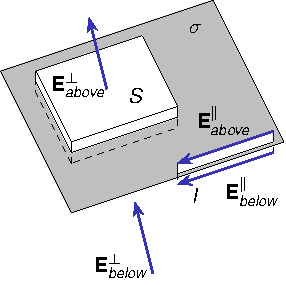
\includegraphics[width=\textwidth]{Figures/Boundary_conditions.pdf}
        \caption{Boundary Conditions.}
        \label{Boudary_conditions}
        \end{figure}
        \vspace{-3mm}
        Metal: \( \varepsilon \rightarrow \infty\). \\
        Supercoductor: \( \mu \rightarrow 0\).

        

\end{columns}
\end{frame}